\chapter{Holonomy Groups}\label{chap4}% chapter 4

\section{Integral paths}\label{chap4:sec1} % section 4.1

We\pageoriginale shall consider in this chapter only connected base manifolds.

\setcounter{defn}{0}
\begin{defn}\label{chap4:sec1:def1}% definition 1
  A {\em{path}} $\psi$ in a manifold $W$ is a continuous map $\psi$ of
  the unit interval $I =[0,1]$ into $W$. A path $\psi$ is said to be
  {\em{differentiable }} if $\psi$ can be extended to a differentiable
  map of an open neighbourhood of $I$ into $W$. $\psi(0)$ is called
  the origin and $\psi (1)$ the extremity, of the path. The path $t
  \rightarrow \psi(1-t)$ is denoted by $\psi^{-1}$. If $\gamma$ is a
  connection on a principal bundle $P$ over $X$, then a differentiable
  path $\psi$ in $P$ is said to be {\em{integral}} if  $\psi^* \gamma
  = 0$. If $\psi$ is integral, so is $\psi^{-1}$. 
\end{defn}

Let $\psi$ be a path in $X$. A path $\hat{\psi}$ in $P$ such that $po
~\hat{\psi} = \psi$ is called a lift of $\psi$. It is easy to see that
if $\hat{\psi}$ is an integral lift of $\psi$, so is $\hat{\psi} s$,
where $\hat{\psi} s$  is defined by  $\hat{\psi} s (t) =
\hat{\psi}(t)s$. If $\hat{\psi}$ is an integral lift of $\psi$, then
$\hat{\psi}^{-1}$ is an integral lift of $\psi^{-1}$. 

\setcounter{theorem}{0}
\begin{theorem}\label{chap4:sec1:thm1}%theorem 1
  If $\psi$ is a differentiable path in $V$ with origin at $x \in V$,
  then for every $\xi \in P$  such that $p(\xi) = x$, there exists one
  and only one integral lift of $\psi$ with origin $\xi$. 
\end{theorem}

Let $I'$ be an open interval containing $I$ to which $\psi$ can be
extended.\pageoriginale The map $\psi : I' \rightarrow V$ defines an induced bundle
$P_\psi$ with base $I'$ and a canonical homomorphism $h$ of $P_\psi$
into $P$ such that the diagram 
\[
\xymatrix@R=1.5cm@C=1.5cm{P_\psi \ar[d]_q \ar[r]^h & P \ar[d]_p\\
I' \ar[r]^\psi & V}
\]
is commutative. The connection $\gamma$ on $P$ also induces a
connection $h^* \gamma$ on $P_\psi$. Since $I'$ is a curve, by Ex.1
of Ch.\ref{chap3:sec7} and Th.\ref{chap3:sec6:thm5} of Ch.3.6, there
exists a section $\sigma$ 
such that the inverse image by $\sigma$ of $h^* \gamma$ is zero. i.e. $\sigma^*
h^* \gamma = 0$. Define $\hat{\psi}: I' \rightarrow P$ by setting
$\hat{\psi} = h \sigma$ on $I'$. Then it is obviously an integral lift
of $\psi$. If $s \in G$ is such that $\xi = \hat{\psi}(0)s$, then
$\hat{\psi} s$  is an integral lift of $\psi$ with origin $\xi$. 

If $\hat{\varphi},\hat{\psi}$ are two such lifts, then we may define a
map $s : I \rightarrow G$ such that  
$$
\hat{\psi}(t) = \hat{\varphi}(t)s(t) \text{ for every } t \in I.
$$

Since $\hat{\varphi},\hat{\psi}$ are differentiable, it can be proved
that $s$ is also differentiable using the local triviality of the
bundle. Differentiation of the above yields $\hat{\psi} (dt) =
\hat{\varphi}(dt) s(t) + \hat{\varphi}(t) s(dt)$. Hence 
$$
\gamma(\hat{\varphi}(dt)s(t)) + \gamma (\hat{\varphi}(t) s(dt)) = 0.
$$

Using conditions (1) and (2) of connection form, we get $s(dt) =
0$. Hence $s$ is a constant. Since $\hat{\varphi}(0) = \hat{\psi}(0)$,
the theorem is completely\pageoriginale proved. 

\section{Displacement along paths}\label{chap4:sec2}%section 4.2

Let $P_x$ be the fibre at $x$ and $\psi$ a path with origin $x$ and
extremity $y$. For every $\xi \in P_x$, there exists one and only one
integral lift $\hat{\psi}$ of $\psi$ whose origin is $\xi$. The
extremity of $\hat{\psi}$ is an element of the fibre at $P_y$. We
shall denote this by $\tauup_\psi \xi$. Then $\tauup_\psi$ is said to
be a displacement along $\psi$. Any displacement along the path $\psi$
commutes with the operations of $G$ in the sense that $\tauup_\psi
(\xi s) = (\tauup_\psi \xi) s$ for every $\xi \in P_x$; therefore
$\tauup_\psi$ is differentiable and is easily seen to be a bijective
map  $P_x \rightarrow P_y$. Trivially, $(\tauup_\psi)^{-1} =
\tauup_{\psi^{-1}}$. It is also obvious that the displacement is
independent of the parameter, i.e., if $\theta$ is a differentiable
map of $I$ into $I$ such that  
\begin{enumerate}[1)]
\item $\theta (0) = 0, \theta(1) = 1$;
\item $\psi' \theta = \psi$
\end{enumerate}
then $\tauup_{\psi'} = \tauup_\psi$

Given a differentiable path $\psi$, we may define a new path $\psi'$
by suitably changing the parameter so that $\psi'$ has all derivatives
zero at origin and extremity. By the above remark, we have
$\tauup_{\psi^{-1}} = \tauup_\psi$. 

\section{Holonomy group}\label{chap4:sec3}% section 4.3

\begin{defn}\label{chap4:sec3:def2}% definition 2
  A chain of paths in $V$ is a finite sequence of paths $\{\psi_p$,
  $\ldots, \psi_1 \}$ where $\psi_i$ is a path such that $\psi_{i + 1}
  (0) = \psi(1)$ for $i \le p-1$. 
\end{defn}

We define the origin and extremity of the chain $\psi$ to be
respectively\pageoriginale $\psi_1(0)$ and  $\psi_p(1)$. Given two chains 

 $\psi = \{ \psi_p, \psi_{p-1} ,\ldots \psi_1\}, \varphi =\{
\varphi_q, \varphi_{q-1}, \ldots \varphi_1 \ 
\}$ such that origin of $\psi=$ extremity of $\varphi$, we define
$\psi \varphi = \{ \psi_p, \ldots \psi_1, \varphi_q , \ldots \varphi_1
\}$. $\varphi^{-1}$ is defined to be $\{ \varphi^{-1}_1, \ldots
\varphi^{-1}_q \}$ and it is easily seen that $(\psi \varphi)^{-1}=
\varphi^{-1} \psi^{-1}_1$.

A displacement $\tau_{\psi}$ along a chain $\psi = \{ \psi_p, \ldots
\psi_1 \}$ in the base manifold $V$ of a principal bundle $P$ is
defined by $\tau_{\psi}= \tau_{\psi p }\circ , \ldots \circ \tau_{\psi
  1}$. 

Let $x, y \in V$. Define $\Phi (x, y)$ to be the displacements
$\tau_{\psi}$ where $\psi$ is a chain with $\psi (0) =x, \psi (1) =
y$. It can be proved, by a suitable change of parameters of the paths
$\psi_i$ (ch. \ref{chap4:sec2}), that there exists a differentiable path $\varphi$
such that $\tau_{\varphi} = \tau_{\psi}$. The following properties are
immediate consequences of the definition: 
\begin{enumerate}[1)]
\item $\alpha \in \Phi (x,y) \Longrightarrow \alpha^{-1} \in \Phi (y,x)$.
\item  $\alpha \in \Phi (x,y), \beta \in \Phi (y,z) \Longrightarrow
  \beta \alpha \in \Phi (x,y)$. 
\item $\Phi (x,y)$ is non empty since $V$ is connected.
\end{enumerate}

  We shall denote $\Phi (x, x)$ by $\Phi (x)$. $\Phi (x)$ is then a
  subgroup of the group of automorphisms of $P_x$ commuting with
  operations of $G$. This is called the \textit{ holonomy group } at
  $x$ with respect to the given connection on the principal bundle
  $P$. If we restrict ourselves to all chains homotopic to zero at
  $x$, then we get a subgroup $\Phi_r (x)$ of $\Phi (x)$, viz., the
  subgroup of displacements $\tau_{\psi}$ where $\psi$ is a closed
  chain at $x$ homotopic to zero. This is called the
  $\textit{restricted holonomy group}$ at $X$. This is actually a
  normal subgroup of $\Phi (x)$, for if $\psi$ is homotopic\pageoriginale to $0$ and
  $\varphi$ any continuous path $\varphi \psi \varphi^{-1}$ is again
  homotopic to zero. 

\setcounter{proposition}{0}
\begin{proposition}\label{chap4:sec3:prop1}%Prop 1
  For every $x \in V$, there exists a natural homomorphism of the
  fundamental group $\prod _1 (V, x)$ \textit{ onto } $\Phi (x)/
  \Phi_r (x)$. 
\end{proposition}

Let $\psi$ be a closed path at $x$. Then there exists a differentiable
path $\psi'$ homotopic to $\psi$. We map $\psi$ on the coset of
$\Phi_r (x)$ containing $\tau_{\psi 1}$. If $\varphi$ and $\psi$ are
homotopic, so are $\varphi'$ and $\psi'$ i.e. $\psi' \varphi'^{-1}$ is
homotopic to zero. Then $\tau_{\psi' \varphi' -1} = \tau_{\psi},
\tau^{-1}_{\varphi} \in \Phi_r$. Thus we obtain a canonical map
$\theta : \prod_1 (V, x) \to \Phi(x) / \Phi_r (x)$ which is easily
seen to be a homomorphism of groups. That this is surjective is
immediate. 

In general, $\theta$ will not be injective. As the fundamental group
of manifolds which are countable at $\infty$ is itself countable, so
is$ \Phi(x) / \Phi_r (x)$. Hence from the point of view of structure
theory, a study of $\Phi_r(x)$ is in most cases sufficient. 

\section{Holonomy groups at points of the bundle}\label{chap4:sec4}%Sec 4.4

If $x, y$ are two points of the connected manifold $V$ and $\varphi$ a
path joining $x$ and $y$, then there exists an isomorphism $\Phi (y)
\to \phi(x)$ defined by $\tau_{\psi} \to \tau_{\varphi -1} \tau_{\psi}
\tau_{\varphi}$ for every path closed at $y$. The image of
$\Phi_r(y)$ under this isomorphism is contained in $\Phi_r
(x)$. However, this isomorphism is not canonical depending as it does
on the path $\varphi$. The situation can be improved by association
to each point of the bundle $P$ a holonomy group which is a subgroup
of $G$. 

Let $A_x$ be the group of automorphisms of $P_x$ commuting with
operations\pageoriginale of $G$. Let $\xi \in P_x$, Then we define an isomorphism
$\lambda_{\xi}: A_x \to G$ by requiring $\alpha \xi = \xi
\lambda_{\xi}(\alpha)$ for every $\alpha \in A_x$. That $\lambda
_{\xi}$ is a homomorphism and is bijective is trivial. At every $\xi
\in P$, we define the \textit{ holonomy group} $\bar{\varphi}(\xi)$ to
be $\lambda_{\xi} \Phi (p \xi)$. Similarly the \textit{restricted
  holonomy group} $\Phi_r (\xi) $ at $\xi $ is $\lambda_{\xi} \Phi_r
(p \xi)$.  

\begin{theorem}\label{chap4:sec4:thm2}%Thm 2
\end{theorem}

For any two points $\xi , \eta \in P, \Phi (\xi) , \Phi (\eta)$ are
conjugate subgroups of $G$. Moreover, if $\xi , \eta$ lie on an
integral path, then $\Phi (\xi) = \Phi(\eta)$. 

If $\xi, \eta$ are on the same integral path, then $\eta = \tau
\varphi \xi$ for some path $\varphi$ with origin $p \xi =x$ and
extremity $p \eta= y$. It is sufficient to prove that $\Phi(\xi)
\subset \Phi (\eta)$. Let $\psi$ be a closed chain at $x$. Then 
\begin{align*}
  \xi(\lambda_{\xi} \tau_{\psi}) & = \tau_{\psi} \xi\\
  & = \tau_{\psi} \tau_{\varphi}^{-1} \eta\\
  &= \tau_{\varphi}^{-1} \tau_{\psi}' \eta \text{ where } \psi' =
  \varphi \psi \varphi^{-1}\\ 
  & = \tau_{\varphi}^{-1}( \eta \lambda_{\eta}( \tau_{\psi'}))\\
  & = \xi \lambda_{\eta}(\tau_{\psi}')
\end{align*}
Hence $\lambda_{\eta} (\tau_{\psi'}) = \lambda_{\xi}(\tau_{\psi}) \in
\Phi (\eta)$ and our assertion is proved. 

Finally, if $\xi , \eta$ are arbitrary, we may join $p \xi, p \eta$ by
a path $\varphi$. Let $\hat{\varphi}$ be an integral lift of $\varphi$
through $\xi$ and $\eta'$ its extremity. Then there exists $s \in G$
such that $\eta' = \eta s$. We have\pageoriginale already proved that $\Phi (\xi) =
\Phi (\eta s)$. Now  
\begin{align*}
  (\eta s) (\lambda_{\eta s} (\alpha)) & = \alpha (\eta s)\\
  & = (\eta \lambda_{\eta}(\alpha)) s
\end{align*}
Hence $\Phi(\xi) = s^{-1} \Phi (\eta)s$, which completes the proof of
theorem \ref{chap4:sec4:thm2}. 

\section{Holonomy groups for induced connections}\label{chap4:sec5}%Sec 4.5

Let $h$ be a homomorphism of a principal bundle $P'$ over $V'$ into a
principal bundle $P$ over $V$. Let $h$ be the projection of
$h$. Let $\gamma$ be a connection form on $P$ and $h* \gamma$ the induced
connection on $P'$. If $\xi' \in P'$ and $h (\xi') = \xi$, then
$\Phi(\xi') \subset \Phi (\xi)$. 
Moreover, $\Phi (\xi')$ is the set of $\lambda_{\xi}(\tau_{h_{\psi'}})$
where $\psi'$ is a closed chain at $p \xi'=x'$. For, let $s \in
\Phi(\xi')$ corresponding to the closed chain $\psi'$ at $x'$.  Then
$\xi' s = \tau_{\psi '} \xi'$. 
\begin{align*}
  \xi s & = h (\tau_{\psi '} \xi')\\
  &= \tau_{\psi} \xi \quad \text{ where } \quad \psi = \underbar{h} \psi'\\
  &= \xi \lambda_{\xi}(\tau_{\psi}).
\end{align*}

Therefore $s = \lambda_{\xi}(\tau_{\psi})$ and it is obvious that any
such $\lambda_{\xi}(\tau_{\psi})$ belongs to $\Phi (\xi')$. 

In particular, let $V'$ be the universal covering manifold of $V,
\underbar{h}$ the covering map, $P'$ a principal bundle over $V'$ and
$h$ a homomorphism $P' \to P$ whose projection is $\underbar{h}$. Then
for $\xi \in P'$, $\Phi(\xi')$\pageoriginale is the set of $\lambda_{\xi}
\tau_{\psi}$ where $\psi$ is the image under $\underbar{h}$ of a
closed chain at $p \xi'$. But $V'$ being simply connected, $\psi$ is
any closed chain at $\xi$ homotopic to zero and hence $\Phi (\xi') =
\Phi_r (\xi)$. 

\section{Structure of holonomy groups}\label{chap4:sec6}%Sec 4.6

\begin{theorem}\label{chap4:sec6:thm3}%Thm 3
\end{theorem}
For every $\xi \in P, \Phi_r (\xi)$ is an arcwise connected subgroup of $G$.

If $\psi$ is a closed path at $x \in V$ which is homotopic to zero,
then it can be shown that there exists a \textit{ differentiable} map
$\varphi : I' \times I' \to V(I'$ being a neighbourhood of $I$) such
that $\varphi (t, 0) = \psi (t)$ and $\varphi(t, 1) =x$ for every $t
\in I$. This can be lifted into a map $\hat{\varphi}: I' \times I' \to P$
such that  
\begin{enumerate}[1)]
\item $p \hat{\varphi} (t , \theta ) = \varphi (t, \theta)$ for every
  $t, \theta \in I$; 
\item For every $\theta \in I, t \to \hat{\varphi} (t , \theta )$ is
  an integral path; 
\item $\hat{\varphi} (0 , \theta ) = \xi$ with $p (\xi ) =x$.
\end{enumerate}

In fact, $\varphi: I' \times I' \to V$ induces a bundle $P_{\varphi}$
over $ I' \times I'$. Let $\gamma_{\varphi}$ be the induced connection
on $P_{\varphi}$. For every $\theta \in I'$, the path $t \to (t,
\theta)$ in $ I' \times I'$ can be lifted to an integral path
$\hat{\sigma}_{\theta}$ in $P_\phi$ with origin at $((0, \theta) , \xi) \in
P_{\varphi}$. The origin depends differentiably on $\theta$ and
therefore the map $\sigma$ of $ I' \times I'$ defined by $\sigma(t,
\theta) = \sigma_{\theta}(t) $ is differentiable. Hence $\rho\circ  \sigma
= \hat{\varphi}$ satisfies the conditions $1),2)$ and $3)$. 

Now we define a function $s : I \to G$ by requiring that $\xi
s(\theta) = \hat{\varphi} (1, \theta)$. Obviously $s(1) =e$ and $s(0)$
is the element of\pageoriginale the restricted holonomy group at $\xi$ corresponding
to the path $\psi$. It is also easy to verify that $s(\theta)$ is a
differentiable function of $\theta$ using the local triviality of
$P$. Therefore any point of $\Phi_r (\xi)$ can be connected to $e$ by
a differentiable arc. 

\begin{coro*}%Corlry
  $\Phi_r (\xi)$ is a Lie subgroup of $G$.
\end{coro*}

This follows from the fact that any arcwise connected subgroup of a
Lie group is itself a Lie group \cite{31}. 

\section{Reduction of the structure group}\label{chap4:sec7}%Sec 4.7

\begin{theorem}\label{chap4:sec7:thm4}%4
\end{theorem}

The structure group of $P$ can be reduced to $\Phi (\xi)$ for any $\xi \in P$.

For this we need the following 

\setcounter{lem}{0}
\begin{lem}\label{chap4:sec7:lem1}%Lem 1
  Let $M(\xi)$ be the set of points $\xi'$ of $P$ which are
  extremities of integral paths emanating from $\xi$. There exists an
  open covering $(U_i)_{i \in I} $ of $V$ and cross-sections
  $\sigma_i$ over $U_i$ such that $\sigma_i (x) \in M (\xi)$ for every
  $x \in U_i$. 

  Let $x = p \xi$ and $x_0 \in V$. Consider the path $\psi$ connecting
  $x$ and $x_0$. Then the integral lift $\hat{\psi}$ of $\psi$ with
  origin $\xi$ has extremity $\xi_0$ with $p \xi_0 = x_0$. Let $U$ be
  a neighbourhood of $x_0$ in which are defined $n$ linearly
  independent vector fields $\underbar{X}_1, \ldots \underbar{X}_n$
  where $n = \dim V$. Let $X_1 , X_2, \ldots X_n$ be horizontal vector
  fields on $p^{-1}(U)$ such that $pX_i =  \underbar{X}_i$ for every
  $i$. By the theorem on the existence of solution for differential
  equations, there exists a neighbourhood of $(0, 0, \ldots)$ in $R
  \times R^n$ in which is defined a differentiable map $\xi$ having
  the properties  
  
  \begin{enumerate}[1)]
  \item $\xi(0,a) = \xi_0$\pageoriginale
  \item $\xi'(t, a) = \sum t a_i (X_i)_{\xi (t, a)}$.
  \end{enumerate}
\end{lem}

From the uniqueness of such solutions, we get 
$$
\xi (\lambda t,a) = \xi(t, \lambda a)
$$
for sufficiently small values of $\lambda, t$ and $a$. Thus there
exists a differentiable map $\xi$ having the properties $1)$ and $2)$
above on $[0, 2] \times W$ where $W$ is a neighbourhood of $(0,
\ldots)$ in $R^n$. Since the $X_i$ are horizontal, $\xi (t, a) \in
M(\xi)$. Now consider the differentiable map $g : W \to P$ defined by
$g(a) = \xi (1, a)$. The map $p.g$ is of maximal rank. Moreover since
$\dim V = n$, this is locally invertible. In other words, in a
neighbourhood $U'$ of $X_0$ we have a differentiable map $f :U' \to W$
such that $p \circ g \circ f$ = Identity, i.e., gof is a cross section over $U$,
and  
$$
(\text{ gof }) \,(y) = \xi (1, f(y)) \in M (\xi) ~~\text{ for every }~~ y \in U'.
$$

\setcounter{proof of theorem}{3}
\begin{proof of theorem}% Prf of thm 4
  We have only to take for transition functions the functions $m_{ij}$
  such that  
  $$
  \sigma_i(x) = \sigma_j (x) m_{ji}(x) ~~\text{ for every } ~~x \in
  U_i \cap U_j 
  $$
  where the $\sigma_i$ have the properties mentioned in the lemma. Then
  it is obvious that $m_{ij}(x) \in \Phi(\sigma_i(x_0)) = \Phi(\xi)$
  by theorem \ref{chap4:sec4:thm2}, Ch. 4.3. 
\end{proof of theorem}

Now let $V$ be simply connected. Then $\Phi (\xi) = \Phi_r
(\xi)$. Since $\Phi(\xi)$ is a Lie subgroup of $G$, it follows \cite{11}
that the $m_{ji}$\pageoriginale are differentiable functions as maps: $U_i \cap U_j
\to \Phi (\xi)$ also. 
If $\rho_i$ are the diffeomorphisms $U_i \times G \to p^{-1} (U_i)$
defined by $\rho_i(\xi, s) = \sigma_i(\xi)$s for $\xi \in U_i, s \in
G$. Consider the set $W_i$ consisting of $\rho_i(\xi, s)$ with $\xi
\in U_i, s \in \Phi (\xi)$. It is clear that $W_i \cap p^{-1}(U_j) =
W_j \cap p^{-1} (U_i)$. Moreover if we provide each $W_i$ with the
structure of a differentiable manifold by requiring that the $\rho_i$
be a diffeomorphism, then the differentiable structures on $W_i \cap
W_j$ agree. In other words, $M (\xi) = \bigcup \limits_{i \in I} W_i$
has a differentiable structure (with which it is a submanifold of
$P$). $\Phi (\xi)$ acts on $M (\xi)$ differentiably to the right and
makes of it a principal bundle over $V$ with projection $p$. We denote
the inclusion map $M (\xi) \to P$ by $f$.

\begin{proposition}\label{chap4:sec7:prop5}%Prop 5
  Let $d \eta$ be a vector at the point $\eta$ of the manifold
  $M(\xi)$ and $\mathscr{Y} (\xi)$ the Lie subalgebra of $\mathscr{Y}$
  corresponding to $\Phi (\xi)$, then $\gamma(fd \eta) \in \mathscr{Y}
  (\xi)$. 
\end{proposition}

Since the connection form is $0$ on horizontal vectors, it is enough
to consider the case when $f d \eta$ is tangential to the fibre,
i.e. is of the form $sa$ with $a \in \mathscr{Y}(\xi), s \in
\Phi(\xi)$. In this case $\gamma (sa) = a \in \mathscr{Y} (\xi)$ which
proves the assertion. 

If we define $\gamma^* (d \eta) = \gamma (fd  \eta)$ for every vector
$d \eta$ of $M(\xi)$ then $\gamma^*$ is again a connection form on the
principal bundle $M(\xi)$. For every point $\eta \in M(\xi)$, the
holonomy group corresponding to $\gamma^* $ is $\Phi (\xi)$. 

\section{Curvature and the holonomy group}\label{chap4:sec8}%Sec 4.8

\begin{theorem}\label{chap4:sec8:thm5}%thm 5
\end{theorem}
For $\xi \in P, \Phi_r (\xi) = (e)$ if and only if the curvature form
is\pageoriginale identically zero. 

Consider the universal covering manifold $\tilde{V}$ of $V$ with
covering map $\underbar{h}$. Let $\tilde{P} = P_{\underbar{h}}$ be the
induced bundle with $h$ as the homomorphism $\tilde{P} \to P$. Let
$\tilde{\xi} \in \tilde{P}$ such that $h \tilde{\xi} = \xi$. Then by
Ch.\ref{chap4:sec5}., the holonomy group $\Phi (\tilde{\xi})$ with respect to the
induced connection $\tilde{\gamma}= h^* \gamma$ on $\tilde{P}$ is
$\Phi_r (\xi)$. Therefore, if $\Phi_r (\xi)= (e), M(\tilde{\xi})$ is the
image of a cross-section $\tilde{\sigma}$ of $\tilde{P}$ over $V$. By
prop. \ref{chap3:sec6:prop4}, Ch.3.6, $\tilde{\gamma}\tilde{\sigma}(d~\tilde{x})=0$ for every
$\tilde{x}\in \tilde{V}$. Hence by th.\ref{chap3:sec6:thm5}, Ch.3.6 the curvature is
0. Since $\tilde{V}$ is locally diffeomorphic with $V$ the
curvature form of $\gamma$ is $0$. Conversely, if $K=0, \tilde{K} =0$
and by th.\ref{chap3:sec6:thm6}, ch.3.6, there exists a section $\tilde{\sigma}$ of
$\tilde{P}$ over $\tilde{V}$ such that $\tilde{\gamma} \tilde{\sigma}=0$ and
such that $\tilde{\sigma}(\tilde{x})= \tilde{\xi}$. Hence the holonomy
group at $\tilde{\xi}$ reduces to $\{ e\}$, i.e., $\Phi_r (\xi) = \{ e
\}$. 

\begin{theorem}[Ambrose-Singer; \cite{1}]\label{chap4:sec8:thm6}%Thm 6
\end{theorem}

The Lie algebra of the restricted holonomy group $\Phi_r (\xi)$ at $\xi
\in P$ is the subspace of the Lie algebra $\mathscr{G}$ of $G$
generated by the values $K(d_1 \eta,\break d_2 \eta)$ of the curvature form
with $d_1 \eta, d_2 \eta \in T_{\eta}, \eta \in f M(\xi)$. 
We may assume that $V$ is simply connected in which case $\Phi (\xi) =
\Phi_r (\xi)$, the general case being an easy consequence. Moreover,
since it is enough to take $d_1 \eta, d_2 \eta$ to be horizontal, we
may consider the values of $K$ on the manifold $M(\xi)$. We may
therefore restrict ourselves to the case when $\Phi_r (\xi) = G$, and
$M(\xi) =P$. Let $\mathscr{I}$ be the \textit{ subalgebra } of
$\mathscr{G}$ generated by the values of $K$. Let $\mathscr{L}$ be the
set of vector fields $X$ on $P$ such that $\gamma (X)$ is a function
with values in $\mathscr{I}$. This is an $\mathscr{U}(P)$-
submodule. It is easily seen that $\mathscr{L}$ has everywhere rank\pageoriginale$=
\dim V + \dim \mathscr{I}$, using the fact that $\gamma (Z_a)=a \in
\mathscr{I}$ for $a \in \mathscr{I}$. Moreover, 
\begin{align*}
  \gamma ([X, Y]) \xi & = -K(X, Y) \xi- X \gamma (Y) \xi + Y \gamma (X)
  \xi + [ \gamma (X) , \gamma (Y) ] \xi\\ 
  & \in \mathscr{I} ~\text{ for every }~  X, Y \in \mathscr{L}~
  \text{ and }~ \xi \in P. 
\end{align*}

By Frobenius' theorem, there exists an integral manifold for the
distribution given by $\mathscr{L}$. Let $L$ be the maximal integral
manifold for $\mathscr{L}$ containing $\xi$. Since the integral paths
for $\gamma$ with origin at $\xi$ are integral with respect to
$\mathscr{L}$ we must have $L = P$. Hence $\dim \mathscr{I} = \dim
\mathscr{G}$, or $\mathscr{I} = \mathscr{G}$.  

Finally it remains to prove that the subspace $\mathscr{M}$ of
$\mathscr{U}$ generated by the values of $K$ is itself a Lie
subalgebra. 

Since $K(d_1 \eta s, d_2 \eta s) = s^{-1}K(d_1 \eta , d_2 \eta) s \in
\mathscr{I}$, it follows that $s^{-1} \mathfrak{N} s \subset
\mathfrak{N}$ for every $s \in G$. Therefore for every $X \in
\mathscr{I}, [X, \mathfrak{N}] \subset \mathfrak{N}$. In particular,
$[\mathscr{M},\mathscr{M}] \subset \mathscr{M}$. 

We now give a geometric interpretation of $K(d_1 \xi , d_2 \xi)$ for
$\xi \in P$. Firstly, we may assume $d_1 \xi , d_2 \xi$ to be both
horizontal vectors (Prop. \ref{chap3:sec6:prop3}, Ch.3.6). Let $x = p \xi, d_1 x = pd_1
\xi$ and $d_2 x = pd_2 \xi$. Extend $d_1 x , d_2 x$ to vector fields
$\underbar{X}_1$ and $\underbar{X}_2$ on $V$ such that $[
  \underbar{X}_1, \underbar{X}_2] =0$. Let $X_1, X_2$ be the
corresponding projectable, horizontal vector fields on $P $. Let $\eta
\to F_i (\eta, t)$ be the automorphism of parameter $t$ defined on a
neighbourhood of $\xi$ by the vector field $X_i (i=1, 2)$. We set
$\xi_1(\theta) = F_1 (\theta , \xi), \xi_2 (\theta) = F_2 (\theta,
\xi_1(\theta)), \xi_3(\theta) = F_2(-\theta, \xi_2(\theta))$ and
$\xi_4 (\theta) =F_1 (-\theta, \xi_3 (\theta))$. The chain of paths
$F_1(t/ \theta, \xi)$, $F_2(t/ \theta , \xi_1 (\theta)), F_1 (-t/
\theta , \xi_2 (\theta))$, $F_2(-t / \theta , \xi_3 (\theta))$\pageoriginale is not
closed in general though its projection on $V$ is closed (since $[X_1,
  X_2] =0)$. 
Let $s(\theta^2)$ be the element of $G$. such that $\xi_4 (\theta) =
\xi s (\theta^2)$. Then $[X_1, X_2]_{\xi} = \xi s'(0)$ and we have  
\begin{align*}
  [X_1, X_2]_{\xi} & = \gamma([X_1, X_2]_{\xi})\\
  & = -K(X_{1 \xi}, X_{2 \xi})\\
  & = -K(d_{1 \xi}, d_{2 \xi}).
\end{align*}
\begin{figure}[H]
\centering{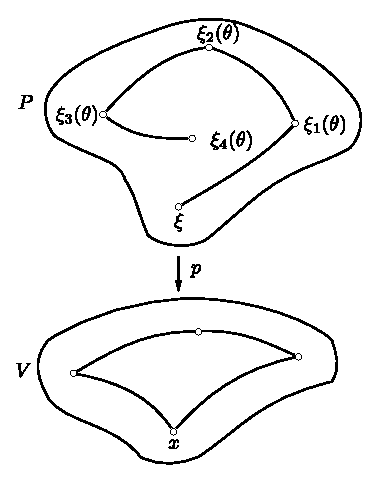
\includegraphics{vol20-figures/fig20-1.eps}}
\end{figure}
